\subsection{Chili sin carne}

% source: https://www.theseriousgut.com/blogs/news/chili-sin-carne-vegan-anti-inflammatoire

\culabel{chili-sin-carne}{4}

\begin{center}
	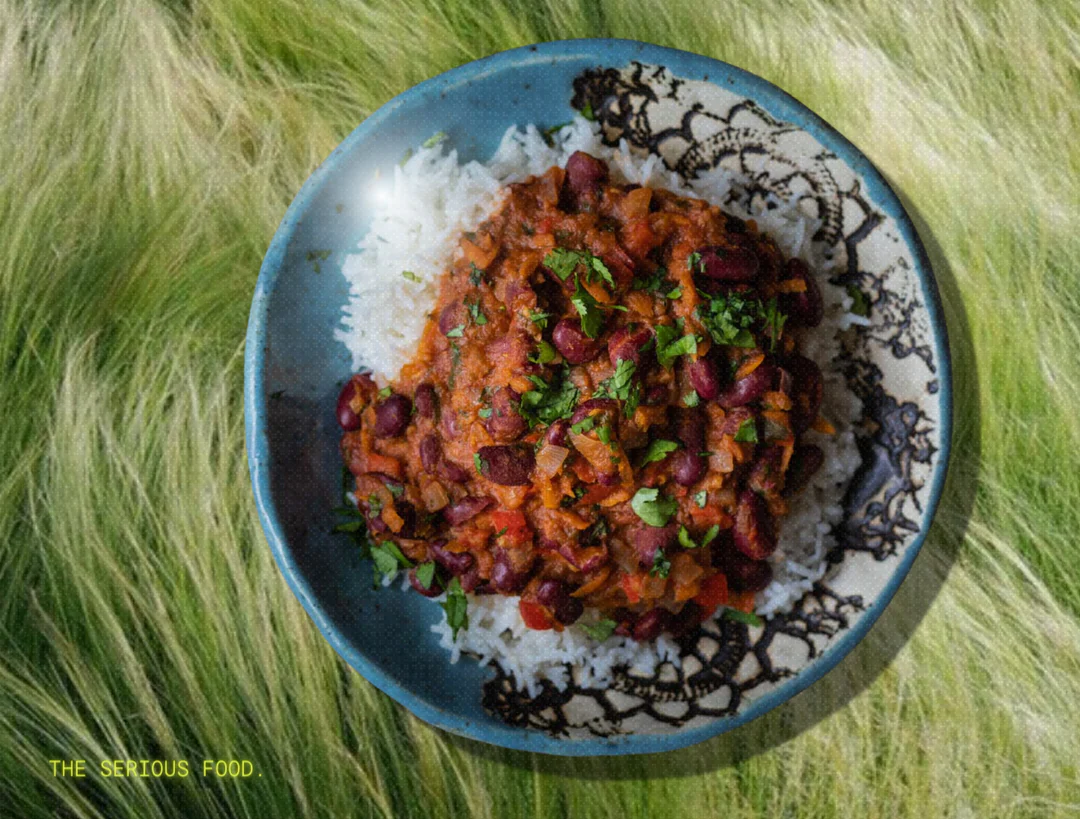
\includegraphics[clip,height=3cm,width=0.8\linewidth]{./img/chili-sin-carne.png}
\end{center}

\subsubsection*{À propos}

\begin{center}
	\begin{tabularx}{0.8\linewidth}{|c|X|c|c|} \hline
		Type & Temps & Pour & Matériel \\ \hline
		Plat & 1 heure (dont 50 minutes de cuisson) & \curef{chili-sin-carne} personnes & \Gasstove \\ \hline
	\end{tabularx}
\end{center}

\subsubsection*{Ingrédients}

\begin{multicols}{2}
	\begin{itemize}
		\item Haricots rouges \cunum<chili-sin-carne>{300}{g} \index{Haricot rouge}
		\item Oignon \cuam<chili-sin-carne>{1} \index{Oignon}
		\item Gousse d'ail \cuam<chili-sin-carne>{1} \index{Ail}
		\item Cumin \cunum<chili-sin-carne>{1}{EL} \index{Cumin}
		\item Huile d'olive \index{Huile d'olive}
		\item Origna \cunum<chili-sin-carne>{1}{EL} \index{Origan}
		\item Paprika \cunum<chili-sin-carne>{1}{EL} \index{Paprika}
		\item Coriandre \index{Coriandre}
		\item Sel
		\item Poivre
		\item Tomates pelées \cunum<chili-sin-carne>{500}{g} \index{Tomate}
		\item Poivron rouge \cuam<chili-sin-carne>{1} \index{Poivron rouge}
		\item Riz complet \index{Riz}
	\end{itemize}
\end{multicols}

\subsubsection*{Préparation}

\begin{enumerate}
	\item Peler et émincer finement l'ail et l'oignon.
	Laver le poivron et le couper en lanières.
	\item Dans une cocotte ou une grande casserole, faire revenir l'ail et l'oignon dans un peu d'huile d'olive (pas trop chaud).
	Faire revenir jusqu'à ce que l'oignon devienne translucide.
	\item Ajouter les haricots égouttés et laisser cuire \cutext{5}{min}.
	\item Ajouter les tomates pelées et toutes les épices, la coriandre ciselée, saler et poivrer.
	\item Laisser mijoter \cutext{45}{min} (ou plus).
	Ajouter un peu d'eau si besoin.
	\item Servir bien chaud avec du riz complet.
\end{enumerate}
